\documentclass[letterpaper,9pt,a4paper]{article}
\usepackage{ulem}
\usepackage{url}

\usepackage{epsfig}
\usepackage{graphicx,color}% Include figure files
\usepackage{wrapfig,caption}
\usepackage{epstopdf}

\usepackage{fancyhdr,graphicx,epsfig,lastpage}
\usepackage{amsmath}
\usepackage{amssymb}

\usepackage{latexsym}
\usepackage[latin1,applemac]{inputenc}

%\usepackage{natbib}

\usepackage{booktabs}



\usepackage{mdwlist}
%\usepackage{enumitem}

%\usepackage[sort&compress,sectionbib]{natbib}
% \usepackage{german,isolatin1}
\usepackage{indentfirst}
%\usepackage{natbib}

\setlength{\parindent}{0in}
%\usepackage[superscript]{cite}

\usepackage{setspace} % Allows spacing of sections with \singlespacing and \doublespacing command

\oddsidemargin 0pt 
\evensidemargin 0pt 
\marginparwidth 68pt 
\marginparsep 10pt 
\topmargin 0pt 
\headheight 0pt 
\headsep 5pt

\voffset -40pt 
\footskip 0pt 
\textheight 25cm 
\textwidth 16.8cm 
\columnsep 10pt 
\columnseprule 0pt 
\sloppy 
%\frenchspacing

\linespread{1.27}

%\setlength{\parindent}{0pt} 
%\setlength{\parskip}{5pt plus 2pt minus 1pt}
%\renewcommand{\baselinestretch}{1.095} %{1.2} %{1.095}
%\clubpenalty=5000 \widowpenalty=5000
%\renewcommand{\footnoterule}{\vspace{0.5cm}%
%  \rule{2.5in}{0.4pt} \vspace{0.3cm}} \pagestyle{fancy}
%\renewcommand{\headrulewidth}{0.4pt} \lhead{Research Plan} \chead{}
%\rhead{\today} \renewcommand{\footrulewidth}{0.4pt} \lfoot{}
%\cfoot{\thepage /\pageref{LastPage}} \rfoot{}

%%%%%%%%%%%%%%%%%%%%%%%%%%%%%%%%%%%%%%%%%%%%%%%%%%%%%%%%%
% Main
%%%%%%%%%%%%%%%%%%%%%%%%%%%%%%%%%%%%%%%%%%%%%%%%%%%%%%%%%
\begin{document}
%\noindent
\begin{center}

  %\textbf{\Large Research Plan}\\[10mm]

%  \textbf{Title:}\\[5mm]
% \textbf{\Large Measuring Incentives for Attacks \& Security, }\\[4mm]
% \textbf{\Large and Managing Cyber Risk}\\ [10mm]

  %{\today}\\[85mm]

  %\textbf{PhD candidate:}\\
 % \textbf{\large Thomas Maillart}\\[10mm]

  %\textbf{Advisor:}\\
  %Prof. Dr. Didier Sornette\\
  %Chair of Entrepreneurial Risks\\
  %ETH Z\"urich (Swiss Federal Institute of Technology in Z\"urich)\\[5mm]

  % \textbf{Co-referee:}
  % \\[5mm]
  

\vspace{-1cm}
{\large {\bf \textsc{Characterizing Contribution Strategies and Quality \\ with Bi-Partite Networks in Wikipedia\\}}}
\begin{center}
\vspace{-0.cm}
\footnotesize{order of preference : (1) talk, (2) ignite talk, (3) poster}
\end{center}
\vspace{-0.cm}
{ {\bf \textsc{Maximilian Klein, Thomas Maillart, John Chuang}}}
\vspace{0.2cm}
\end{center}

\vspace{0.05cm}
According to the adage {\it ``given enough eyeballs, all bugs are shallow"} \cite{raymond1999}, open source projects achieve high quality from the variety of edits performed by many contributors. We aim to test this adage by characterizing the contribution strategies by editors in $12$ categories of Wikipedia articles, using networks models with two node types: articles and editors. The {\it biased random walk} method in bi-partite networks \cite{caldarelli2012network} is a reflexive method, in which produced entities are ranked as a function of producing entities, and conversely in a recursive way \cite{hidalgo2009}. This approach is a two node-type version of the {\it pageRank} algorithm \cite{page1999pagerank} and compares to a random walker jumping between editors and articles (see Figure \ref{fig1}A). Jumps are controlled by parameters $\alpha$ and $\beta$, which determine the probability to jump from editors to articles with more links (resp. from articles to editors with more links). When $\alpha$ or $\beta$ equal zero, this indicates an equal probability to jump to a neighboring node. However, larger $\alpha$ (resp. $\beta$) indicates a lower probability to jump to a node with more links. In other words, for a node of a given type, $\alpha$ (or $\beta$ depending on the node type) controls the importance of the connectivity of neighboring nodes with nodes of same type as the original one. $\alpha$ or $\beta$ therefore provide direct information on the structure of influence between articles and editors.

\begin{figure}[h]
\centering
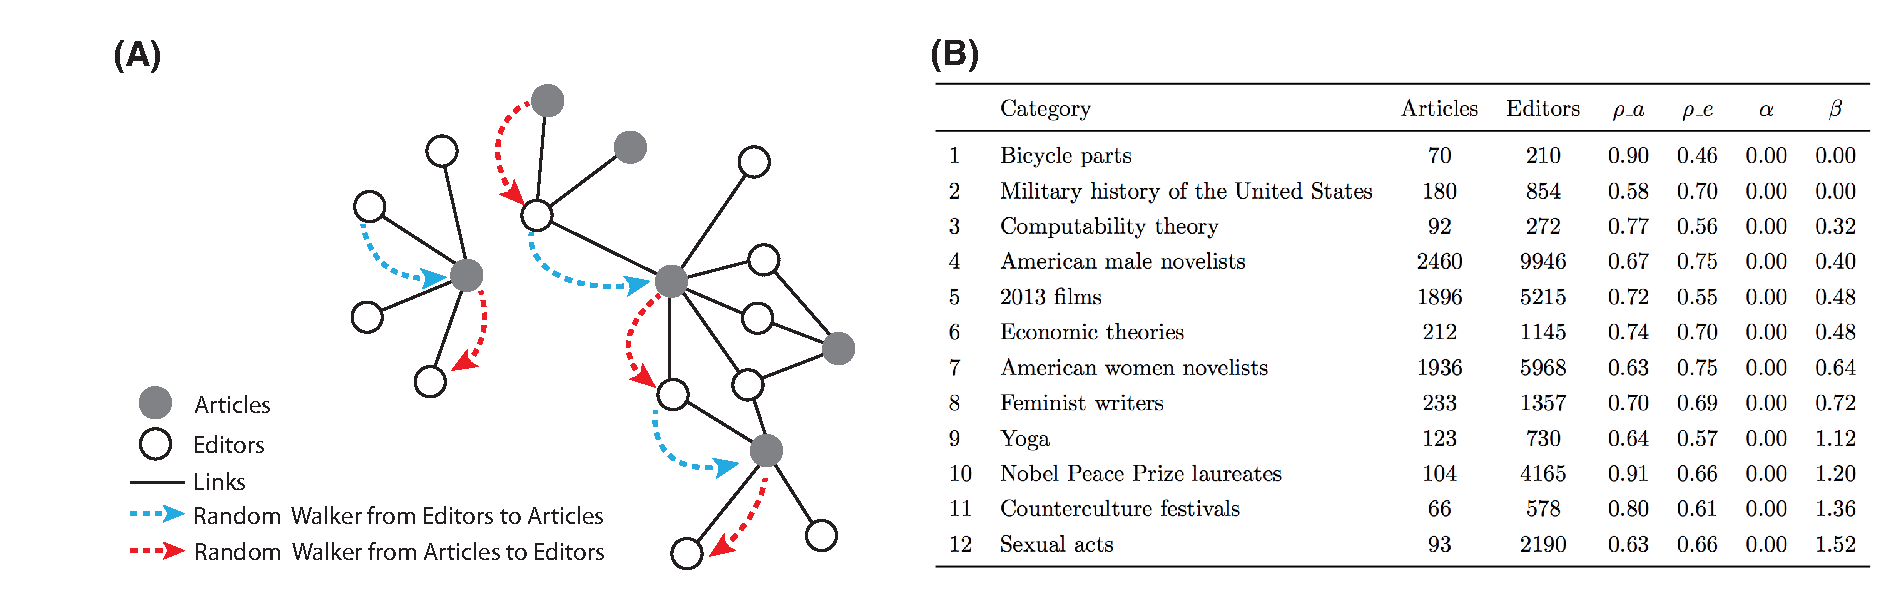
\includegraphics[width=1.\columnwidth]{Figures/figure_abstract.eps}
\caption{\footnotesize {\bf (A)} Bi-partite network with Article and Editor nodes. Dashed arrows show how the random walker jumping between articles and editors with  probability controlled by the appropriately biased connectivity of the each node. {\bf (B)} Table shows the best rank-correlation $\rho_a$ and $\rho_e$ of the algorithm with the ground truth for each Wikipedia category, as well the value of the divestment bias $\beta$.}
\label{fig1}
\end{figure}

Calibration of $\alpha$ and $\beta$ by maximizing rank-correlation with ground-truth quality metrics for editors and articles shows that the bi-partite random walker} model of influence accounts particularly well for both quality of articles ($0.58 < \rho_a < 0.91$) and expertise of editors ($0.46 < \rho_e < 0.75 $). The best rank-correlation is obtained for $\alpha= 0$ and $0 \leqslant \beta \leqslant 1.52$ (c.f. Figure 1B). Since $\alpha = 0$, articles always benefit from scrutiny by more editors, hence confirming the famous adage. However, for categories with $\beta >0$ the quality of an article is also negatively influenced by the portfolio size of its editors. In other words, when $\beta$ is large, the more articles an editor edits, the lower his or her contributed value to one single article. $\beta$ also characterizes each category and the way quality is achieved through the cumulative contribution of information. For $\beta$ small, all editors have a fairly equal chance to contribute positively to any article, while for $\beta$ large, an editor can only contribute positively to a subset of articles (the larger $\beta$ the smaller the set). Typically, it is unlikely for a single person to have visited all {\it counterculture festivals}, performed all {\it sexual acts} or {\it Yoga} practices, while it is easier for anyone to gather relevant information on {\it bicycle parts} or the {\it US military history}. In conclusion for $\beta > 0$, Raymond's adage should be appended in the following way : {\it ``given enough eyeballs, all bugs are shallow. But each pair of eyeballs cannot kill all bugs"}.


%\begin{tabular}{llcccccc}
%\toprule
%         &                     Category & Articles & Editors & $\rho_a$ & $\rho_e$ & $\alpha$ & $\beta$ \\
%\midrule
% 1&                        Bicycle parts &       70 &     210 &     0.90 &     0.46 &     0.00 &    0.00 \\
% 2&Military history of the United States &      180 &     854 &     0.58 &     0.70 &     0.00 &    0.00 \\
%  3&                Computability theory &       92 &     272 &     0.77 &     0.56 &     0.00 &    0.32 \\
%   4&            American male novelists &     2460 &    9946 &     0.67 &     0.75 &     0.00 &    0.40 \\
%    5&                        2013 films &     1896 &    5215 &     0.72 &     0.55 &     0.00 &    0.48 \\
%     6&                Economic theories &      212 &    1145 &     0.74 &     0.70 &     0.00 &    0.48 \\
%     7&         American women novelists &     1936 &    5968 &     0.63 &     0.75 &     0.00 &    0.64 \\
%     8&                 Feminist writers &      233 &    1357 &     0.70 &     0.69 &     0.00 &    0.72 \\
%     9&                             Yoga &      123 &     730 &     0.64 &     0.57 &     0.00 &    1.12 \\
%     10&      Nobel Peace Prize laureates &      104 &    4165 &     0.91 &     0.66 &     0.00 &    1.20 \\
%      11&        Counterculture festivals &       66 &     578 &     0.80 &     0.61 &     0.00 &    1.36 \\
%        12&                   Sexual acts &       93 &    2190 &     0.63 &     0.66 &     0.00 &    1.52 \\
%\bottomrule
%\end{tabular}



\bibliographystyle{Science}
\bibliography{tmaillart}  

\end{document}
